\documentclass[preprint,journal]{vgtc}       % preprint (journal style)

%% Uncomment one of the lines above depending on where your paper is
%% in the conference process. ``review'' and ``widereview'' are for review
%% submission, ``preprint'' is for pre-publication, and the final version
%% doesn't use a specific qualifier. Further, ``electronic'' includes
%% hyperreferences for more convenient online viewing.

%% Please use one of the ``review'' options in combination with the
%% assigned online id (see below) ONLY if your paper uses a double blind
%% review process. Some conferences, like IEEE Vis and InfoVis, have NOT
%% in the past.

%% Please note that the use of figures other than the optional teaser is not permitted on the first page
%% of the journal version.  Figures should begin on the second page and be
%% in CMYK or Grey scale format, otherwise, colour shifting may occur
%% during the printing process.  Papers submitted with figures other than the optional teaser on the
%% first page will be refused.

%% These three lines bring in essential packages: ``mathptmx'' for Type 1
%% typefaces, ``graphicx'' for inclusion of EPS figures. and ``times''
%% for proper handling of the times font family.

\usepackage{mathptmx}
\usepackage{graphicx}
\usepackage{times}
\usepackage{color}
\usepackage{bm}
\usepackage{amsmath}
\usepackage{siunitx}


%% We encourage the use of mathptmx for consistent usage of times font
%% throughout the proceedings. However, if you encounter conflicts
%% with other math-related packages, you may want to disable it.

%% allow for this line if you want the electronic option to work properly
\vgtcinsertpkg

%% Paper title.

\title{Muscular fascicle arrangement based on Laplacian vector fields}

%% This is how authors are specified in the journal style

%% indicate IEEE Member or Student Member in form indicated below
\author{Jan Kusterer, Niven Ratnamaheson, Raimund Rolfs, and Tobias Walter}
\authorfooter{
%% insert punctuation at end of each item

}

%other entries to be set up for journal
%\shortauthortitle{Schmid \MakeLowercase{\textit{et\,al.}}: ProjINF for fun and profit}

%% Abstract section.
\abstract{
} % end of abstract

%% Keywords that describe your work. Will show as 'Index Terms' in journal
%% please capitalize first letter and insert punctuation after last keyword
\keywords{muscle, fascicle, mesh, Laplace, electrostatic, streamline}

%% ACM Computing Classification System (CCS).
%% See <http://www.acm.org/class/1998/> for details.
%% The ``\CCScat'' command takes four arguments.

\CCScatlist{ % not used in journal version
	\CCScat{Computer Graphics}{I.3.8}{Applications}{Molecular Dynamics Visualization}
	\CCScat{Simulation and Modeling}{I.6.6}{Simulation Output Analysis}{Molecular Dynamics Visualization}
	\CCScat{Computer Graphics}{I.3.7}{Three-Dimensional Graphics and Realism}{Raytracing}
}

\graphicspath{{pics/}}

%% Uncomment below to include a teaser figure.
\teaser{
\centering
\includegraphics[width=12cm]{triceps.png}
\label{fig:teaser}
}

%%%%%%%%%%%%%%%%%%%%%%%%%%%%%%%%%%%%%%%%%%%%%%%%%%%%%%%%%%%%%%%%
%%%%%%%%%%%%%%%%%%%%%% START OF THE PAPER %%%%%%%%%%%%%%%%%%%%%%
%%%%%%%%%%%%%%%%%%%%%%%%%%%%%%%%%%%%%%%%%%%%%%%%%%%%%%%%%%%%%%%%%

\begin{document}
\maketitle
%% The ``\maketitle'' command must be the first command after the
%% ``\begin{document}'' command. It prepares and prints the title block.

%% the only exception to this rule is the \firstsection command
\section{Introduction}\label{sec:intro}
Skeletal muscles have a wide range of anatomical architectures. 
They often form a heterogenous curvature, while the tendon and bone attachments vary in their morphology~\cite{Choi2013}. 
Each muscle consists of multiple muscle fibers which can contract via Myosin motors, according to Jiangcheng et al. 
\cite{Jiangcheng2015}, and thus create a force pulling on the bones. 
Each motor is organized as a chain of contractile parts, called sarcomeres. 
The fibers are not long enough to cover the whole muscle, so they are grouped in paralleled bundles called fascicles. 

According to \cite{Etemadi.et.Al.} the biceps of an athletic individual has around 300.000 muscle fibers, which are single cells approximately 50 \si\micro m in diameter and several centimeters long \cite{Cooper2000}. 
Each fiber has a thick myosin filament and a thin actin filament, which surrounds the myosin. 
During the process of muscle contraction, the actin and myosin filaments slide past each other resulting in shortening of the fiber.

Since the mechanical force is transmitted along the muscle fibers, it is important for biomechanical simulations to obtain an adequate representation of their trajectories. 
In this way we can get much more realistic geometries e.g. of a contracted biceps.
However, this is not a simple task because of the complexity and diversity of the various muscles. 
To simplify the problem by a small degree, we can simulate the fascicles instead of every single fiber.

To simulate the contraction of a muscle we need an approximation of the fascicles, that stretch across the muscle. 
Although we can see them with our bare eyes, it is not possible to determine their pathway using an ordinary CT-scan. 
Therefore, we need a method to calculate the trajectories of these fascicles.
Muscles are often modelled using a lumped-parameter approach that assumes a simplified arrangement of fascicles. 
However, as Choi and Blemker \cite{Choi2013} stated, these models are not able to cover three-dimensional deformations.

One of the more promising approach is using a Laplacian vector field as presented by Choi et al. \cite{Choi2013}. 

The goal of our work is the approximation of Muscle fascicles based on the 3D-model of a muscle, primarily the musculus biceps brachii, with an approach using a Laplacian vector field. 
% TODO	 überleitung, überblick üver folgende Kapitel
Gmsh ~\cite{Geuzaine2009} is a tool for generating 3-D finite element meshes with built in pre- and post processing. 
We use it for multiple reasons as it is free software that features it's own scripting language, which uses code similar to C++ with loops, conditionals and user-defined macros.
We use these features, because they match our needs for Meshing, Simulation and analysis of the Model. 
It can be compiled without the GUI, directly from the command line. 
For other manipulations and computations we use Python.

%
%% \section{Introduction} %for journal use above \firstsection{..} instead
%
%\todo{Cite some stuff: bullshit~\cite{lipsa2011visualization} and simulation~\cite{hocker:084707}.}
%
\section{Methods}
The first step when calculating the streamlines based on a CT-Scan of the muscle is to repair the STL file. 
Small holes in the surface would make it impossible for gmsh to mesh the volume. 
Most of the mesh processing tools (eg. Meshlab, Blender, Microsoft 3D Builder) feature a repair function. % TODO erklären (anhand figure 1?), CT-scan erklären

Since our pipeline is not suited to compute the streamlines for a biceps with a fork included, we need to cut the 3D-model just below the fork and some part from the opposite side.
As a nice side-effect we get a better distribution of the streamlines in the center part of the muscle. %TODO Bild?

The stl-file does not connect the surface triangles with its neighbours. 
Gmsh however needs one big surface to create a volume in which we can compute the streamlines. 
To connect all the small surfaces, we reclassify the mesh with a threshold of 0.
This runs a edge-detection for all triangles with an angle to its neighbour greater than 0 (so basically every neighbour) and we can connect all the detected surfaces to one big surface.

The reclassified muscle can then be reassambled within a gmsh specific script file.
Another step here is to detect the inflow and outflow surfaces for later steps. 
A python programm is used for this detection. 

3D-Meshing the volume is done completely by gmsh. %TODO introduction oder start von methods
 
As stated by Choi and Blemker~\cite{Choi2013}, a Laplacian vector field yields reasonable results when simulating fascicle arrangement. 
Thats why we use a simulation of an electronic field. 
GetDP the solver, used by gmsh, calculates the gradient inside the mesh of the biceps.

To create the streamlines, we apply the streamlines-plugin on the vector-view. 
We than have decent streamlines in the biceps brachii.

With help of another Python script we extract the streamlines from the postprocessing file and write them in a new geo file. 
Merging this file with the original biceps surface displays their arrangement, as can be seen in the titlepicture.
\begin{figure}
	\begin{center}
		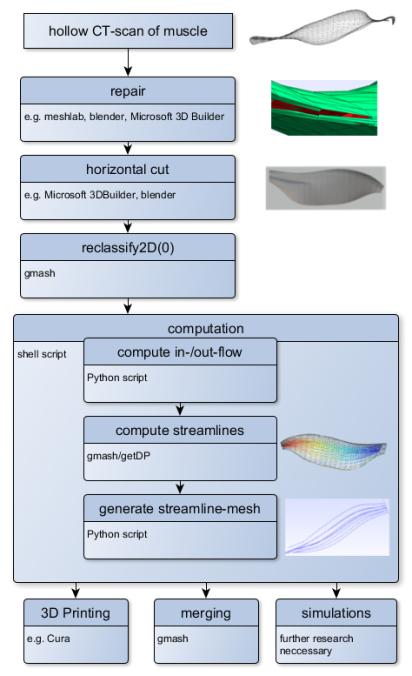
\includegraphics[width=.7\linewidth]{flow.png}
	\end{center}
	\caption{Flowchart of our Pipeline}
	\label{fig:flow}
	
\end{figure}
\section{Preparations}
As we start from a CT-scan we first need to check whether the Volume is complete and closed. 
We noticed little holes in the Surface, as seen  in Figure \ref{fig:holes}, as we tried to Mesh the Volume, which caused gmsh to crash. 
%TODO V Wiederholung?
Therefore we used a Repair feature which most of the common 3D modelling tools share. 
The Biceps, as the name indicates has two heads. 
For easier computation and better outcome of the streamlines, we cut  the muscle horizontal just below the fork and below the main volume. 

\begin{figure}
	\begin{center}
		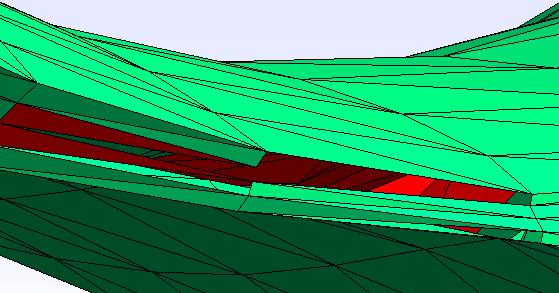
\includegraphics[width = .6\linewidth]{holes.png}
	\end{center}
	\caption{Holes in the forked area of the biceps, which need to be closed. The inside of the biceps is colored red for better contrast.}
	\label{fig:holes}
\end{figure}

\section{Reassembling}
The stl-file does not connect the surface triangles with its neighbours. 
Gmesh however needs one big surface to create a volume in which we can compute the streamlines. 
To connect all the small surfaces, we use the reclassify option with a threshold of 0.
This runs an edge-detection for all triangles with an angle to its neighbour greater than \ang{0}. 
This excludes the two cut surfaces, since these surfaces all have an angle of \ang{0}. 
The prepared muscle is then processed in our pipeline, see Figure ~\ref{fig:flow}. 
Finally we can recombine all the detected surfaces to one big surface. 
The recombination is done within gmsh by iterating over the surfaces and declaring the recombined surface as one. 
The basic operations done in the script are to be seen in ~\ref{code:geo}. 
From all the surfaces, a compound surface is created which then is combined in a surface loop. 
The parametrs used, for example Loop(10000) means that a new loop, with the number 10000 as a name, is defined. 
In the next line, the 10000 is used again to reference the loop, which is then declared as the boundary of a volume with the number 100 as for reference. 

%TODO Werte erklären
\begin{verbatim}
\label{code:geo}
//declare ss as surface
ss[] = Surface {:};
//combine the surfaces
Compound Surface{ss[]};
//create a surface loop
Surface Loop(10000) = {ss[]};
//define the volume inside the loop
Volume(100) = {10000};
//physical entities are needed for simulation
Physical Surface (100) = {ss[]};
Physical Volume ("Body",10) = 100;
//meshing 3D when executing script
Mesh 3;
//disable Automatic Remeshing
Solver.AutoMesh = 0;
\end{verbatim}

With this new reassembled 3D-structure we now run our python script to detect the two cut surfaces. 
Since we cut the biceps orthogonal to the Z-axis of the model, the process is fairly simple.
We look for all vertices with the highest z-coordinate for the upper boundary and the lowest z-coordinate for the lower boundary, respectively.
These two sets are grouped and form two new surfaces. 
With this surface we save the maximum and minimum of the y- and x- coordinates for later use of the streamlines. 
We do this to cover the whole surface with the starting points of the streamlines.
Physical entities are declared as items, that are used in the simulation. 
In this case the two surfaces identified by the python script,the volume and the surface of the muscle are our physical regions. 

%TODO Absätze
\section{Meshing}
Meshing with Gmsh is fairly easy. 
By default Gmsh chooses between three 2D algorithms and two 3D algorithms.
The automatic algorithm selection tries to select the most apropriate for the given structure.

For 2D algorithms there are "MeshAdapt", "Delauny" and the "Frontal" algorithm.
Every one of them has different uses. 
According to Gmsh the "MeshAdapt" works best for very complex, curved surfaces.
"Frontal" is the best choice, when high element quality is important and "Delauny" is fastest for large meshes of plane surfaces.
As stated in the manual for Gmsh the automatic selection chooses "Delauny" for plane surface and "MeshAdapt" for all other surfaces. 

For 3D algorithms there are "Delauny" and "Frontal". 
The “Delaunay” algorithm is the most robust and the fastest. 
However, this algorithm will sometimes modify the surface mesh, and is thus not suitable for producing hybrid structured/unstructured grids.
In that case the “Frontal” algorithm should be preferred. 
As our mesh is unstructured, the "Delauny" is our algorithm. 
The quality of the elements produced by both algorithms is comparable.
For our 3D mesh, first, the 2D surfaces, then the volume is meshed. 
In ~\ref{code:geo} the line "Mesh 3;" is executed, which does exactly this: first, mesh 2D then, mesh 3D.
%\begin{figure}
%	\begin{center}
%		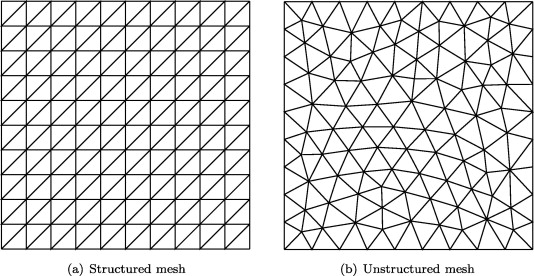
\includegraphics[width=\linewidth]{gridCompare.jpg}
%	\end{center}
%	\caption{Comparisson of structured and unstructured grids ~\cite{}}
%	
%\end{figure}
%-------------------------------------------------------------------------

\section{Simulation}
Our goal is to calculate streamlines of Laplacian vector fields, which according to~\cite{Choi2013} are fairly close to the muscular fascicle arangement. %TODO Wiederholung
Gmsh's solver getDP features a plugin, which calculates the streamlines based on the vector field. 
Therefore we need a simulation on fluid flow or similar. %TODO Gleichungen oder modell erwähnen, ist electrostatic = Laplace?
Electrostatics in a dielectric environment meets the requirement for the Laplace equation, as well as thermodynamics does.
We tried out both thermodynamic and electrostatic simulation. 
In figure ~\ref{fig:L} we see the unsatisfying results we earned using the thermodynamic approach. 
At the corner of the L-figure there are streamlines leaving the Model. 
The result of the electrostatic simulation is spread evenly and has fewer whirls. 
It has a overall better coverage of the model.

The Laplace equation can be used in 3D just as in 2D. 
GetDP's problem definition files (.pro) are used to descripe the models for simulation. 
In this model we consider the calculation of the electric field given a static distribution of electric potential. 
This matches to an "electrostatic" physical model. 
On one end of the muscle we have a conducting surface on top of a dielectric volume, called "Body".
A Dirichlet boundary condition sets the potential on the boundary of the conducting surface , called "Electrode", to 10 mV and to 0 V on the other end of the muscle, called "Ground".
A homogeneous Neumann boundary condition is definded on the surface of the muscle to truncate the domain.

We based our problem definition on the tutorial for electrostatics. ~\cite{Geuzaine2009}
The structure of the file is as follows:

\begin{description}
	\item[Group]
	Start by giving meaningful names to physical regions defined in the mesh file.
	We only use the regions body, electrode and ground. 
	After that we define abstract regions, that are used below.
	\item[Function]
	Here we define material laws.
	\item[Constraint]
	The Dirichlet boundary condtition is defined piecewise. 
	The constraint "Dirichlet\_Ele" is invoked later in the FunctionSpace.
	\item[Group]
	This is the domain definition of The FunctionSpace, which lists al regions on wich a field is defined. 
	The domain contains both the volume and the surface of the muscle.
	\item[FunctionSpace]
	The FunctionSpace is used to pick the electric scalar potential. 
	The solution is defined  by:\newline
	-the domain defenition\newline
	-a type\newline
	-a set of basis functions\newline %TODO welche?
	-a set of entities to wich the basis functions are associated (here all the nodes of the domain)\newline
	-a constraint (here the Dirichlet boundary conditions)
	
	\item[Jacobian] %TODO benötigt?
	Jacobians are used for specifying the mapping of elements in the mesh.
	"Vol" represents the classical 1-to-1 mapping for identical dimension whereas "sur" represents the mapping between 2D and 3D and "lin" is used to map line segments to segments in three dimensional space.
	
	\item[Integration]
	The "Integration" segment specifies how many points are used for the Gauss quadrature rules. %TODO wie viele?
	
	\item[Formulation]
	A GetDP formulation encodes a weak formulation of the partial differential equation. i.e. 
	
	
	\[-\nabla (\varepsilon *\mathrel{grad} v) = 0\]
%	\begin{equation*}
%	\nabla (\varepsilon *grad\ v) = 0
%	\end{equation*}
	
	In our case this weak formulation involves finding v such that
	\[-\nabla \langle \varepsilon *\mathrel{grad} v, v' \rangle _{VolEle}= 0\]
	for all functions v'. $\langle .,. \rangle _{VolEle}$ deotes the inner product over the domain "VolEle". 
	In these equations this domain is our biceps. 
	If v' is differentiable, we usually can find v by using integration by parts with Green's identity:
	\[\langle \epsilon * \mathrel{grad} v, \mathrel{grad} v' \rangle _{VolEle} + \langle n * \epsilon * \mathrel{grad} , v' \rangle _{BndVolEle} =  0\]
	for all v', where "BndVolEle" is the boundary of "VolEle" (the surface of our biceps). 
	In this equation the surface term vanishes, since there is either no function v' or the first factor of the inner product is zero.
	Thus, in our simulation, we are looking for functions v such that 
	\[
	\langle {\epsilon * \mathrel{grad} {v}, \mathrel{grad} v'} \rangle _{VolEle} =  0
	\]
	
	holds for all v'.
	
	The "Integral" statement in the formulation is a representation of this weak formulation. 
	It features four seperated arguements:
	-the density\newline
	-the domain of integration, \newline
	-the Jacobian of the transformation, \newline
	-the integration method to be used.
	
	\item[Resolution]
	In the resolution it is specified what to do with the weak formulation. 
	We simply generate a linear system, solve it and save the solution.  %TODO finite element method??
	\item[Post Processing]
	There are two parts of postprocessing available in getDP. 
	First we can evaluate the outcome of the formulation. 
	Here the quantities are the scalar electric potential, the electric field and the electric displacement.
	The second part are postprocessing operations. 
	In our case the streamline generation is done here. 
	Here the script, which detects the inflow and outflow surfaces, writes the X/Y/Z values so that we get a good coverage of starting points for our streamlines. 
	The operation is then run and the output saved to a postprocessing file (.pos).
	\end{description}

\begin{figure}
	
	\begin{minipage}{\linewidth}
		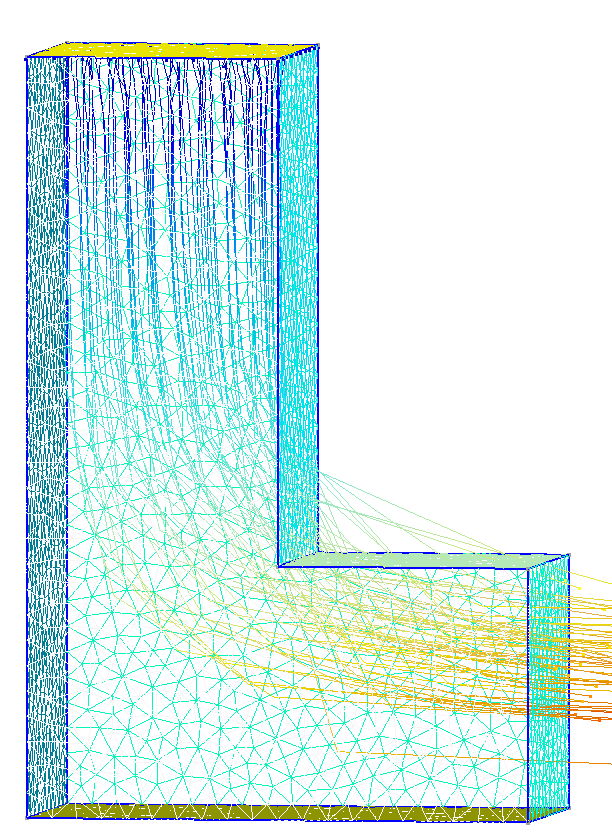
\includegraphics[width=.5\linewidth]{L.PNG} 
		\includegraphics[width=.53\linewidth]{L-ele.png}
		\caption{Comparison of thermodynamic (left) and electrostatic (right) calculation.}
		\label{fig:L}
	\end{minipage}
\end{figure}

\begin{figure}
	\begin{center}
		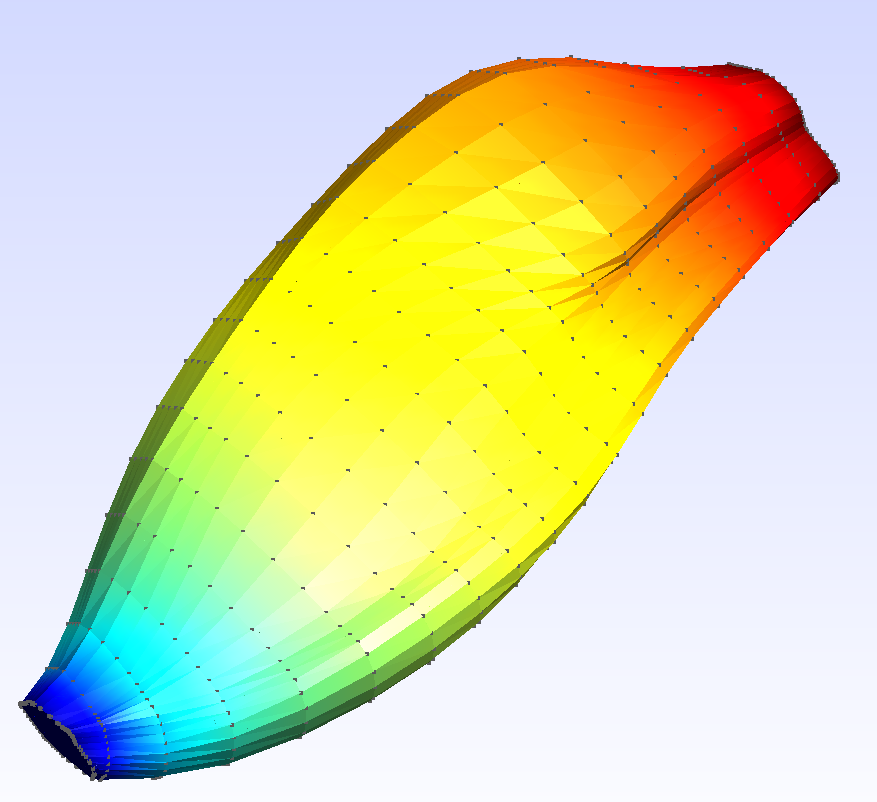
\includegraphics[width=.7\linewidth]{Sim.png}
	\end{center}
	\caption{The cut biceps after the simulation. The colors show the distance from the inflow based on the vector field.}
	\label{fig:sim}
\end{figure}

\section{Streamlines}
We now use the earlier mentioned plugin within the post processing described above, which calculates streamlines. 
The starting points of the streamlines are on the upper surface of the biceps, which was calculated in the reassembling section. 
The number of streamlines can be set when executing the pipeline.
The parameters are given as number of points on the X- and Y- axis. 
The extents of the surface, are the minimal an maximal X and Y values. 
That is why not all of the streamlines will start inside of the muscle. 
Additionally, we can set the number of steps we want to execute  and the length of a step.
The length of the vectors for the streamlines depend on the potential at the point of calculation at that timestep.
Afterwards, instead of extracting the complete streamlines, the exported file only contains the starting point and vectors to each point of the streamlines. 
This however can't be imported into Gmsh since it will only display these vectors and thus we process this data. 

\section{Representation of Data}
Our next step is to add up the vectors of each streamline separately. 
This is done by our python script streamline-converter, which gets the vector data from the muscleStreamline.pos file. 
Furthermore, the script creates a new file streamlines.geo with the data of each streamline in it. 
All in all, we can now use GMSH to merge the streamlines.geo file with our biceps surface to visualize the result. 
However there are multiple ways to represent the streamlines. 
One way to visualize the result is 3D-printing the streamlines.

\section{Printing}
Currently the streamlines are lines without any volume, but to print them they need to be thickened. 
For this step a python script creates points along the streamlines at the target radius resulting in a tube.
The points are then connected and meshed. 
We chose the tubes to have hexagonal profile.
After volume is created all of the streamlines are combined into one stl file. 
Streamlines that lay outside of the biceps will get erased in this step, because they will not have any points in the file. 
The muscle fibers are substracted from the full biceps volume using blender in order to have a hollowed out model with space for the fibers. 
The 3D-Printer we use is the \textit{Ultimaker 3 extended}, which is equipped with two extruders. 
This gives us the option to print with two different materials or colours. %TODO Bild
The software used to pepare printing is Cura. 
We tried printing with a clear material but we didnt get a result, wich allowed the inner setup to be visible. 
We came up with another solution. 
We printed the muscle without the clear material. 
The number of fibres was 7 x 7 when executing our pipeline. 
The printed muscle, however has fewer fibres, as not all of the streamline staring points lay inside the muscle. 
The outcome can be seen in ~ref{fig:printedBiceps}. 

\section{Discussion}
When working with meshes the level of detail plays a key role. 
The model we used was smooth but we noticed a significant increase in quality as we refined the mesh before executing the pipeline. 
As far as refining by splitting goes, we managed to refine the mesh up to two times. 
More splitting was not possible due to Gmsh crashing. 
This increases the amount of nodes by the power of four.
When calculating in the refined setup the streamlines pass way more edges of the thetraeda inside the muscle and as a consequence get a correction in terms of direction and force. 
As a result we recieve smoother streamlines, which cover more space. 
This is to be seen in figure ~\ref{fig:refStreamlines}.

Reclassifying the Mesh is done by hand since Gmsh does not allow reclassifying a mesh by command line with parameters. 
For our Model it is critical to set the threshold to zero. 
This is because Gmsh would see the surface of the muscle as one, when a higher threshold was chosen.

\begin{figure}
	
	\begin{minipage}{\linewidth}
		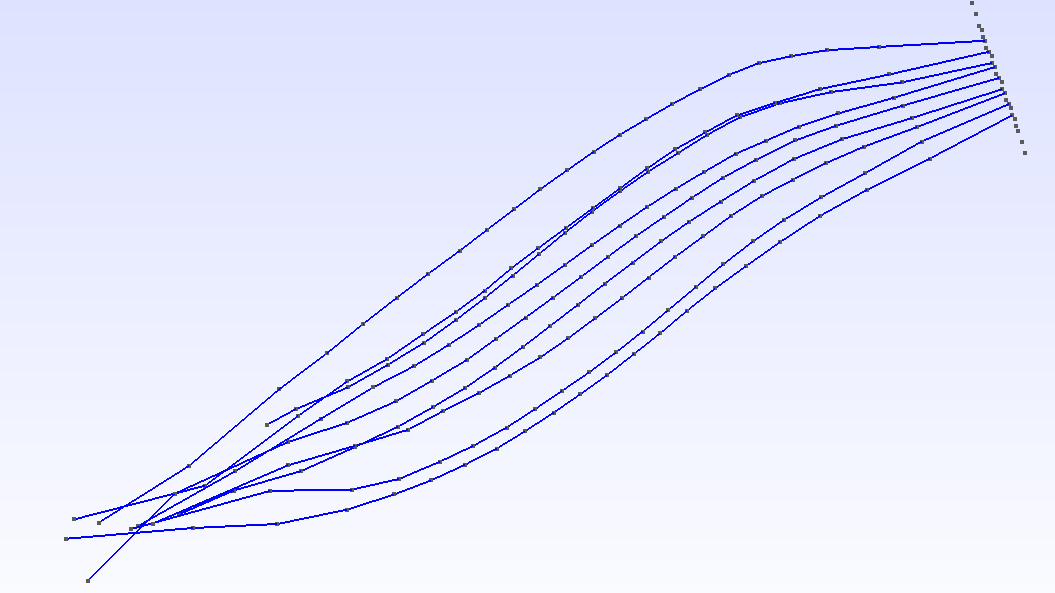
\includegraphics[width=.5\linewidth]{Streamlines.PNG}
		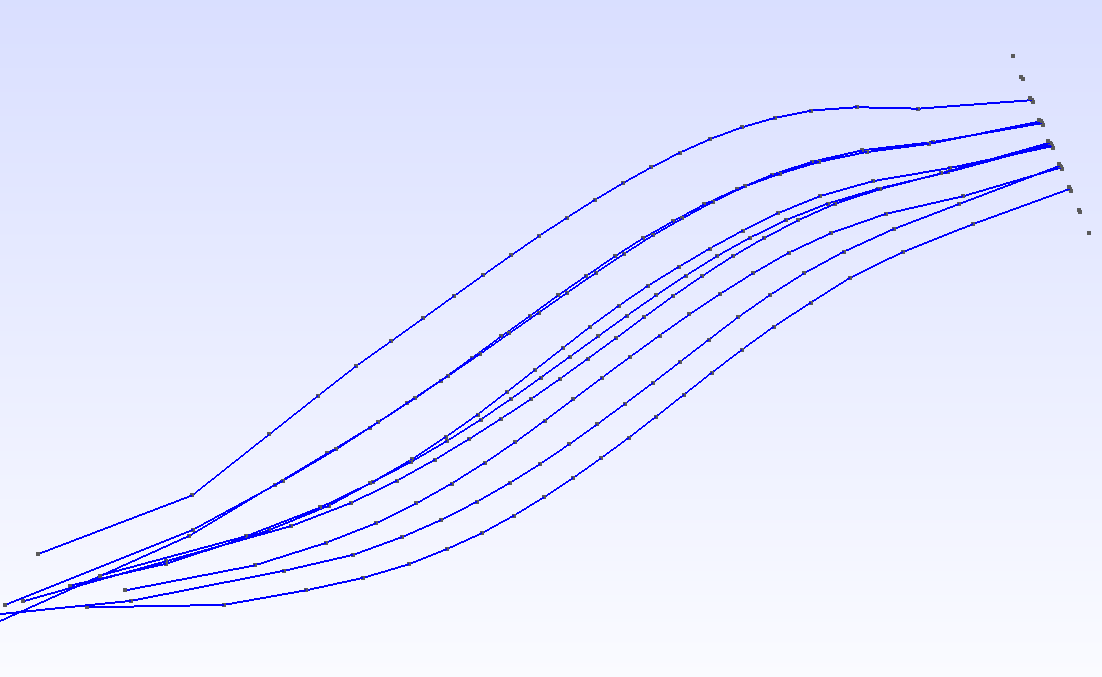
\includegraphics[width=.51\linewidth]{refStreamlines.PNG}
		\caption{Comparison of the two different mesh densities and the resulting resolution of the streamlines. In the right picture the mesh has been refined.}
		\label{fig:refStreamlines}
	\end{minipage}
\end{figure}

\section{Conclusion}


\section{Future work}
-alignment of 3D fascicles with "real thickness"
%% if specified like this the section will be ommitted in review mode
\acknowledgments{
This work was mostly funded by cake and caffein. 

}

\bibliographystyle{abbrv}
%%use following if all content of bibtex file should be shown
%\nocite{*}
\bibliography{documentation}
\end{document} 
